\documentclass[10pt]{article}
\usepackage{graphicx}
\usepackage{float}
\usepackage{amsmath}
\usepackage{amssymb}

\title{Writing of Mathematics}
\author{Atreya Choudhury}

\begin{document}

\maketitle

\section{Introduction}
\textbf{The Problem:}\\
\textit{A dart is thrown at a unit square. The probability of hitting a point closer to the center than to any of the edges equals}

\begin{equation*}
  \frac{4\sqrt{2}-5}{3}
\end{equation*}

We assume \textit{uniform} distribution. Therefore, we can say that the probability of landing the dart on two regions of equal area is equal. To find the probability, we must first find the region where the landing of the dart is acceptable. Then the required probability is the ratio of the areas of target region and the dart board.

\section{The Target}
To define the boundary of the region, we consider those points which are at equal distance from the center of the board and a particular edge. We observe that boundaries are defined by portions of parabolas.

Figure 1 shows the upper right quarter of the board. The red dashed line represents the $1\times1$ board. We set up a co-ordinate system centered at (0,0) co-inciding with the center of the board. The boundaries of the dart-board are:

\begin{align*}
y &= \frac{1}{2}\\
y &= -\frac{1}{2}\\
x &= \frac{1}{2}\\
x &= -\frac{1}{2}
\end{align*}
\newpage
\begin{figure}[H]
\centering
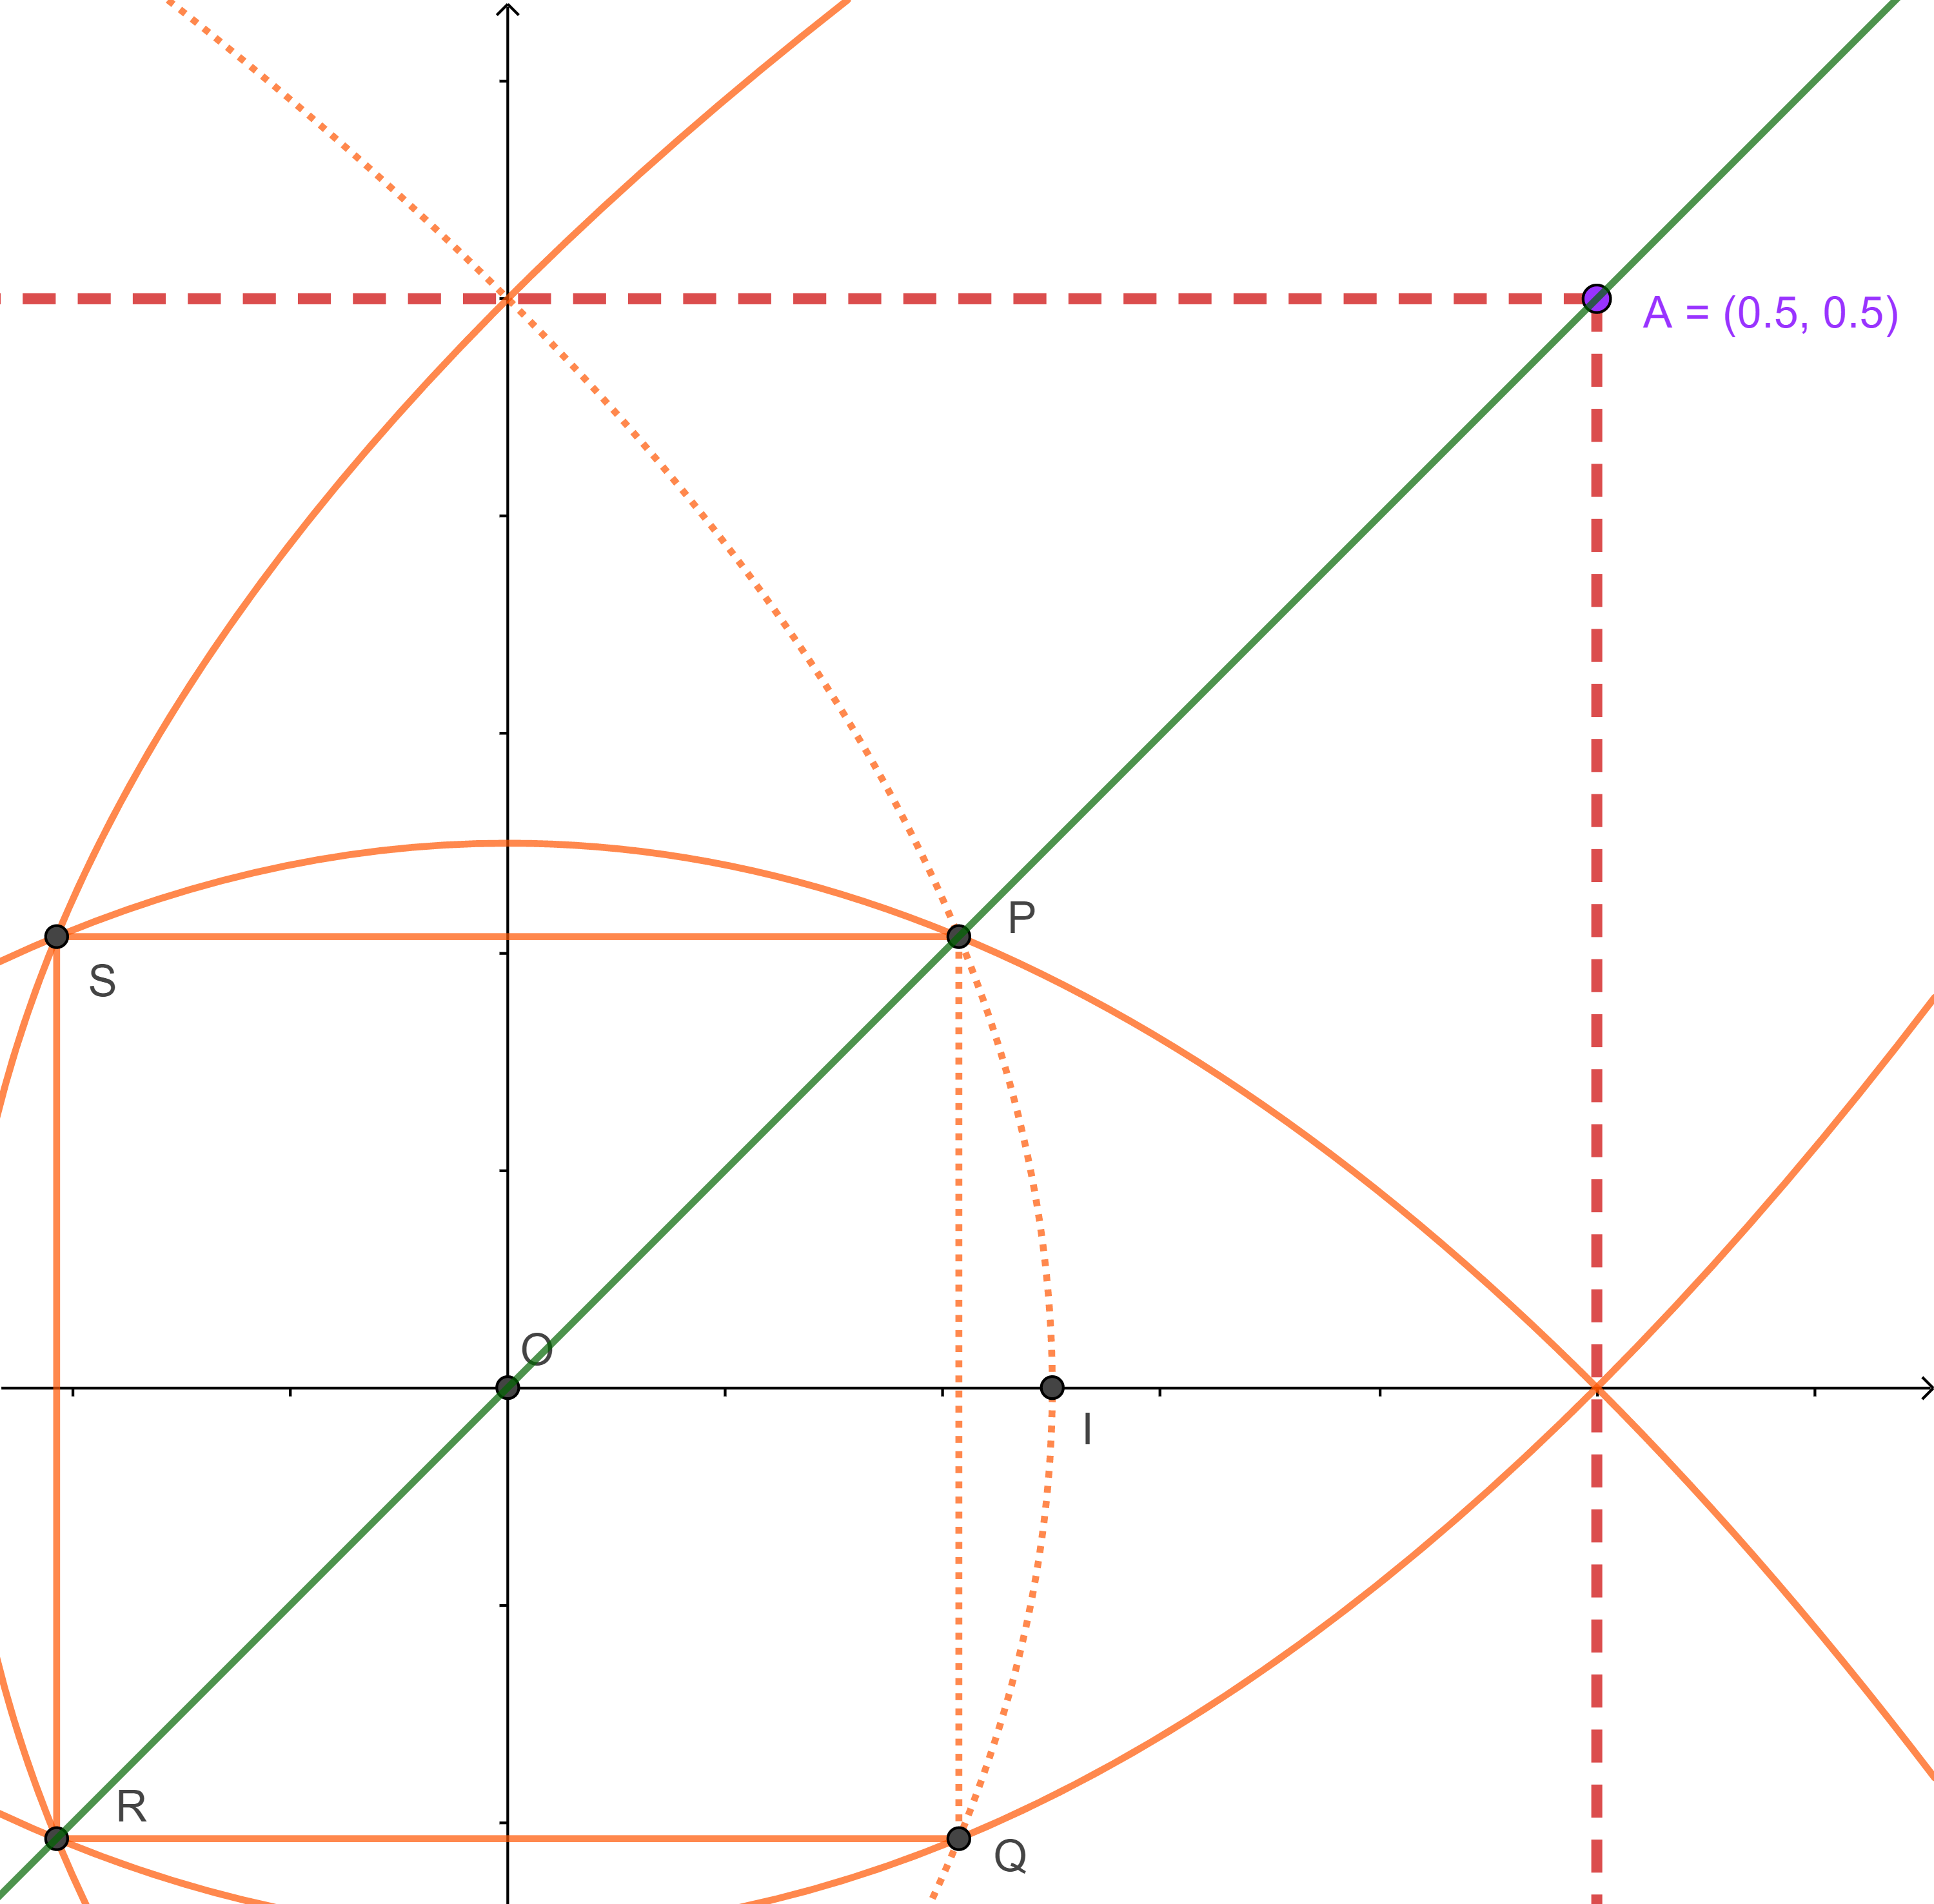
\includegraphics[width = 8cm]{fig1.png}
\caption{Upper Right Quarter of Diagrammatic Representation}
\end{figure}

To calculate the area of the target, we will first find the area of the region enclosed between the orange dotted parabola and the orange dotted side. Then, we can multiply it by 4 (owing to symmetry of the figure) and then add it to the area of the square PQRS.\\

Using the definition of parabolas, the equation of the orange dotted parabola is:

\begin{equation}
\begin{split}
& \therefore \sqrt{{x}^2+{y}^2} = \frac{1}{2} - x\\
&\implies {x}^2+{y}^2 = \frac{1}{4} - x + {x}^2\\
&\implies {y}^2 = \frac{1}{4} - x
\end{split}
\end{equation}
\newpage
To find the co-ordinate of P, we find the intersection of the above parabola with $y = x$.

\begin{equation*}
\begin{split}
& \therefore {x}^2 = \frac{1}{4} - x\\
&\implies {x}^2 + x + \frac{1}{4} = \frac{1}{2}\\
&\implies \left({x + \frac{1}{2}}\right)^2 = \frac{1}{2}\\
&\implies x = - \frac{1}{2} \pm \frac{1}{\sqrt{2}}
\end{split}
\end{equation*}
\\Since, P is in the first quadrant, the co-ordinates of P are $\left(-\frac{1}{2}+\frac{1}{\sqrt{2}}, -\frac{1}{2}+\frac{1}{\sqrt{2}}\right)$
Therefore, the line through P and Q is given by
\begin{equation}
x = - \frac{1}{2} + \frac{1}{\sqrt{2}}
\end{equation}

\section{Area of the Target}
The area enclosed by the orange dotted region is given by:
\begin{equation}
\begin{split}
&2 \times \int_{- \frac{1}{2} + \frac{1}{\sqrt{2}}}^{\frac{1}{4}} \sqrt{\frac{1}{4} - x} \,dx\\
&= 2 \times \Biggl| \frac{-\left({\frac{1}{4} - x}\right)^\frac{3}{2}}{\frac{3}{2}}\Biggr|_{- \frac{1}{2} + \frac{1}{\sqrt{2}}}^{\frac{1}{4}}\\
&= \frac{4}{3} \times \left( \frac{1}{4} - \left(- \frac{1}{2} + \frac{1}{\sqrt{2}}\right) \right)^\frac{3}{2}\\
&= \frac{4}{3} \times \left(\frac{3-2\sqrt{2}}{4}\right)^\frac{3}{2}\\
&= \frac{5\sqrt{2} - 7}{6}\\
\end{split}
\end{equation}

Therefore, the area of the Target Region:

\begin{equation}
\begin{split}
&= \text{Area of PQRS} + 4 \times \text{Area obtained in (3)}\\
&= {(\sqrt{2} - 1)}^2 + 4 \times \left(\frac{5\sqrt{2} - 7}{6}\right)\\
&= \frac{4\sqrt{2} - 5}{3}
\end{split}
\end{equation}
\newpage
\section{Answer and a Small Computation}
The required probability is given by the ratio of the area of the target region obtained in (4) to the area of the dart board which is a unit square.\\

Hence, the probability of landing the dart closer to the center than any edge is $$\frac{4\sqrt{2} - 5}{3}$$\\
which is what we had to prove.\\

I also tried to approximately verify our results by writing a program that generates random co-ordinates, checks if they are in the target region, and calculates the probability accordingly. It generates N such random co-ordinates where N is supplied by the user.\\

\begin{table}[H]
  \centering
  {\renewcommand{\arraystretch}{1.5}
  \renewcommand{\tabcolsep}{0.2cm}
  \begin{tabular}{c|p{1.5 cm}|p{2 cm}|p{3 cm}|p{3 cm}}
    Sl & N & Average Probability & Average Percentage Deviation from the Actual Value & Standard Deviation of Probability from 50 experiments\\
    \hline
    1 & 1,000 & 0.2226 & 5.26587892 & 0.094414\\
    2 & 10,000 & 0.219936 & 1.61945974 & 0.029048\\
    3 & 100,000 & 0.219013 & 0.50371302 & 0.009274\\
    4 & 1,000,000 & 0.218903 & 0.1291184 & 0.0025\\
  \end{tabular}}
  \caption{Probabilities for Experiments with N tries}
  \label{}
\end{table}

\end{document}
